% preamble-exam-zh.tex — 共享 preamble
% 用于所有 exam-zh 模板
%
% 样式策略：
%   屏幕 → 语义彩色（蓝=关键想法，红=易错，绿=路线，灰=提示/教师备注）
%   打印 → 自动降级为黑白（通过 print mode 或 monochrome 选项）

\documentclass{exam-zh}

% ---------- 基础配置 ----------
\examsetup{
  page/size = a4paper,
  page/show-head = false,
  page/show-foot = false,
  sealline/show = false,
  font = times,
  math-font = xits,
}

\usepackage{tcolorbox}
\usepackage{needspace}
\usepackage{graphicx}
\usepackage{tikz}
\usetikzlibrary{calc,arrows.meta,intersections}
\tcbuselibrary{skins,breakable}

% ---------- 打印/屏幕颜色切换 ----------
% 用法：\documentclass[monochrome]{exam-zh} 即可切换为纯黑白
% 注意：不要使用 \if@xxx 放在 makeatother 外部；这里改成普通条件名。
\newif\ifeduprintcolor
\eduprintcolortrue

\makeatletter
\@ifclasswith{exam-zh}{monochrome}{\eduprintcolorfalse}{}
\makeatother

% ---------- 语义颜色定义 ----------
% 屏幕：有色彩区分；打印：降级为灰度
\ifeduprintcolor
  % --- 屏幕彩色模式 ---
  \definecolor{edu-blue}{RGB}{47, 82, 122}       % 关键想法
  \definecolor{edu-blue-bg}{RGB}{243, 246, 252}
  \definecolor{edu-red}{RGB}{180, 40, 40}         % 易错提醒
  \definecolor{edu-red-bg}{RGB}{255, 245, 240}
  \definecolor{edu-green}{RGB}{34, 100, 60}       % 路线图
  \definecolor{edu-green-bg}{RGB}{242, 250, 245}
  \definecolor{edu-orange}{RGB}{160, 90, 0}       % 训练目标
  \definecolor{edu-orange-bg}{RGB}{255, 248, 235}
  \definecolor{edu-gray}{RGB}{100, 100, 100}      % 提示/教师备注
  \definecolor{edu-gray-bg}{RGB}{248, 248, 248}
  \definecolor{edu-purple}{RGB}{90, 50, 120}      % 思考题
  \definecolor{edu-purple-bg}{RGB}{248, 244, 252}
\else
  % --- 打印黑白模式 ---
  \definecolor{edu-blue}{gray}{0.15}
  \definecolor{edu-blue-bg}{gray}{0.96}
  \definecolor{edu-red}{gray}{0.25}
  \definecolor{edu-red-bg}{gray}{0.97}
  \definecolor{edu-green}{gray}{0.20}
  \definecolor{edu-green-bg}{gray}{0.97}
  \definecolor{edu-orange}{gray}{0.25}
  \definecolor{edu-orange-bg}{gray}{0.98}
  \definecolor{edu-gray}{gray}{0.40}
  \definecolor{edu-gray-bg}{gray}{0.97}
  \definecolor{edu-purple}{gray}{0.30}
  \definecolor{edu-purple-bg}{gray}{0.98}
\fi
\colorlet{edu-diagram-muted}{edu-gray}

% ---------- 自定义教学环境 ----------
% 共性：enhanced + breakable（跨页不断裂）

% 原题卡片 — 强边框，突出显示
\newtcolorbox{problemcard}{
  enhanced, breakable,
  colback=edu-blue-bg,
  colframe=edu-blue,
  boxrule=1.2pt,
  arc=0pt,
  left=3mm, right=3mm, top=3mm, bottom=3mm,
}

% 解题路线图 — 左边线 + 浅底
\newtcolorbox{routebox}{
  enhanced, breakable,
  colback=edu-green-bg,
  colframe=edu-green!30,
  boxrule=0pt,
  borderline west={2.5pt}{0pt}{edu-green},
  left=3mm, right=3mm, top=3mm, bottom=3mm,
}

% 关键想法 — 蓝色左边线
\newtcolorbox{keyideabox}{
  enhanced, breakable,
  colback=edu-blue-bg,
  colframe=edu-blue!30,
  boxrule=0pt,
  borderline west={2.5pt}{0pt}{edu-blue},
  left=3mm, right=3mm, top=3mm, bottom=3mm,
}

% 易错提醒 — 红色左边线
\newtcolorbox{mistakebox}{
  enhanced, breakable,
  colback=edu-red-bg,
  colframe=edu-red!20,
  boxrule=0pt,
  borderline west={3pt}{0pt}{edu-red},
  left=3mm, right=3mm, top=2.5mm, bottom=2.5mm,
}

% 提示 — 灰色虚线左边线
\newtcolorbox{hintbox}{
  enhanced, breakable,
  colback=edu-gray-bg,
  colframe=edu-gray!20,
  boxrule=0pt,
  borderline west={2pt}{0pt}{edu-gray, dashed},
  left=3mm, right=3mm, top=2mm, bottom=2mm,
}

% 思考题 — 紫色虚线左边线
\newtcolorbox{thinkbox}{
  enhanced, breakable,
  colback=edu-purple-bg,
  colframe=edu-purple!20,
  boxrule=0pt,
  borderline west={2pt}{0pt}{edu-purple, dashed},
  left=2.5mm, right=2.5mm, top=2.5mm, bottom=2.5mm,
}

% 教师备注 — 灰色左边线，小字
\newtcolorbox{teachernote}{
  enhanced, breakable,
  colback=edu-gray-bg,
  colframe=edu-gray!15,
  boxrule=0pt,
  borderline west={2pt}{0pt}{edu-gray!60},
  left=2.5mm, right=2.5mm, top=2.5mm, bottom=2.5mm,
  fontupper=\small,
  colupper=black!60,
}

% 训练目标 — 橙色左边线，小字
\newtcolorbox{traininggoal}{
  enhanced, breakable,
  colback=edu-orange-bg,
  colframe=edu-orange!15,
  boxrule=0pt,
  borderline west={1.5pt}{0pt}{edu-orange},
  left=2mm, right=2mm, top=1mm, bottom=1mm,
  fontupper=\small,
}

% 答题区 — 无边框，纯留白
\newcommand{\answerarea}[1][40mm]{%
  \vspace{2mm}%
  \begin{tcolorbox}[
    enhanced, breakable,
    colback=white,
    colframe=white,
    boxrule=0pt,
    height=#1,
    valign=top,
    bottom=0mm,
    after skip=0mm,
  ]
  \end{tcolorbox}%
}

\newcommand{\diagramcolfigure}[3]{%
  \begin{minipage}[t]{#2}
    \vspace{0pt}\centering
    \includegraphics[width=\linewidth]{\detokenize{#1}}
    \if\relax\detokenize{#3}\relax\else
      \par\vspace{1mm}{\scriptsize\color{edu-diagram-muted}#3}
    \fi
  \end{minipage}%
}

\newcommand{\diagramrowitem}[4]{%
  \begin{minipage}[t]{#2}
    \vspace{0pt}\centering
    \includegraphics[width=\linewidth]{\detokenize{#1}}
    \if\relax\detokenize{#3}\relax\else
      \par\vspace{1mm}{\scriptsize\bfseries #3}
    \fi
    \if\relax\detokenize{#4}\relax\else
      \par\vspace{0.5mm}{\scriptsize\color{edu-diagram-muted}#4}
    \fi
  \end{minipage}%
}

\newcommand{\answerareawithdiagramcol}[4]{%
  \vspace{2mm}%
  \begin{tcolorbox}[
    enhanced, breakable,
    colback=white,
    colframe=white,
    boxrule=0pt,
    height=#1,
    valign=top,
    bottom=0mm,
    after skip=0mm,
  ]
  \begin{minipage}[t]{\dimexpr\linewidth-#3-6mm\relax}
    \vspace{0pt}
  \end{minipage}\hfill
  \diagramcolfigure{#2}{#3}{#4}
  \end{tcolorbox}%
}

\newcommand{\answerareawithdiagram}[4]{%
  \answerareawithdiagramcol{#1}{#2}{#3}{#4}%
}

% ---------- 字体设置 ----------
% exam-zh (ctexbook) already sets CJK fonts via ctex.
% Only override if specific fonts are needed.
% macOS: Songti SC, STHeiti, STFangsong
% Linux: SimSun, SimHei, FangSong

% ---------- 页面设置 ----------
% exam-zh (ctexbook) already loads geometry.
% Override margins if needed:
% \geometry{top=16mm, bottom=16mm, left=14mm, right=14mm}

\examsetup{
  question/show-answer = false,
  fillin/show-answer = false,
  solution/show-solution = hide,
}

% ---------- 教师版解答样式 ----------
\newtcolorbox{solutionblock}{
  enhanced, breakable,
  colback=edu-blue-bg,
  colframe=edu-blue!25,
  boxrule=0pt,
  borderline west={2pt}{0pt}{edu-blue!50},
  arc=0pt,
  left=3mm, right=3mm, top=2mm, bottom=2mm,
  before skip=2mm,
  after skip=3mm,
  fontupper=\small,
}

% 解答步骤编号
\newcounter{solstep}
\newcommand{\solstep}[2]{%
  \stepcounter{solstep}%
  \par\medskip
  \noindent\hangindent=6mm
  {\color{edu-blue}\bfseries\textcircled{\scriptsize\thesolstep}\enspace #1}\enspace #2\par
}

\begin{document}

\section*{中点四边形练习}

\section*{一、解答题（每题 8 分，共 32 分）}

\needspace{8\baselineskip}

\begin{problem}[points=8]
  如图，四边形 $ABCD$ 中，$E,F,G,H$ 分别是 $AB,BC,CD,DA$ 的中点。判断下列说法是否正确，并说明理由。
\begin{enumerate}[label=(\arabic*)]
  \item 若四边形 $EFGH$ 是矩形，则四边形 $ABCD$ 一定是菱形；
  \item 若四边形 $ABCD$ 是平行四边形，且 $EFGH$ 是矩形，则 $ABCD$ 是菱形。
\end{enumerate}
\begin{center}
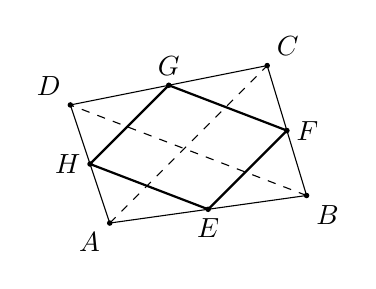
\begin{tikzpicture}[scale=0.5]
  \coordinate (A) at (0,0); \coordinate (B) at (5,0.7); \coordinate (C) at (4,4); \coordinate (D) at (-1,3);
  \coordinate (E) at (2.5,0.35); \coordinate (F) at (4.5,2.35); \coordinate (G) at (1.5,3.5); \coordinate (H) at (-0.5,1.5);
  \draw (A)--(B)--(C)--(D)--cycle;
  \draw[dashed] (A)--(C) (B)--(D);
  \draw[thick] (E)--(F)--(G)--(H)--cycle;
  \foreach \p/\pos in {A/below left,B/below right,C/above right,D/above left,E/below,F/right,G/above,H/left}\fill(\p)circle(2pt)node[\pos]{$\p$};
\end{tikzpicture}
\end{center}

  \answerarea[46mm]
\end{problem}


\needspace{8\baselineskip}

\begin{problem}[points=8]
  如图，在平行四边形 $ABCD$ 中，$E,F,G,H$ 分别是 $AB,BC,CD,DA$ 的中点，四边形 $EFGH$ 是矩形。若 $\angle ABC=120^\circ$，$AC=6\sqrt3$，求平行四边形 $ABCD$ 的周长和面积。
\begin{center}
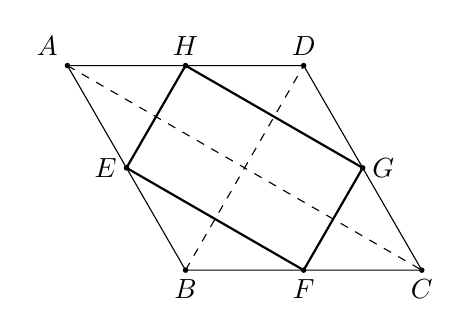
\begin{tikzpicture}[scale=0.5]
  \coordinate (B) at (0,0); \coordinate (C) at (6,0);
  \coordinate (A) at (-3,5.196); \coordinate (D) at (3,5.196);
  \coordinate (E) at (-1.5,2.598); \coordinate (F) at (3,0); \coordinate (G) at (4.5,2.598); \coordinate (H) at (0,5.196);
  \draw (A)--(B)--(C)--(D)--cycle;
  \draw[dashed] (A)--(C) (B)--(D);
  \draw[thick] (E)--(F)--(G)--(H)--cycle;
  \foreach \p/\pos in {A/above left,B/below,C/below,D/above,E/left,F/below,G/right,H/above}\fill(\p)circle(2pt)node[\pos]{$\p$};
\end{tikzpicture}
\end{center}

  \answerarea[50mm]
\end{problem}


\needspace{8\baselineskip}

\begin{problem}[points=8]
  如图，在平行四边形 $ABCD$ 中，$E,F,G,H$ 分别是 $AB,BC,CD,DA$ 的中点，四边形 $EFGH$ 是菱形，且 $EF=5$，$AB=6$。求平行四边形 $ABCD$ 的周长和面积。
\begin{center}
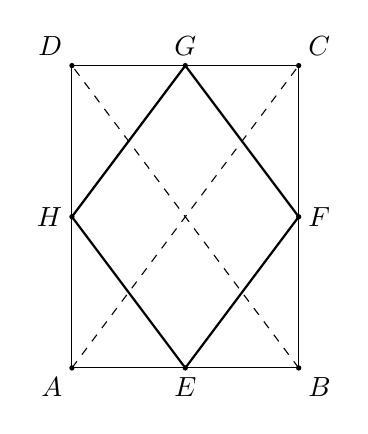
\begin{tikzpicture}[scale=0.48]
  \coordinate (A) at (0,0); \coordinate (B) at (6,0); \coordinate (C) at (6,8); \coordinate (D) at (0,8);
  \coordinate (E) at (3,0); \coordinate (F) at (6,4); \coordinate (G) at (3,8); \coordinate (H) at (0,4);
  \draw (A)--(B)--(C)--(D)--cycle;
  \draw[dashed] (A)--(C) (B)--(D);
  \draw[thick] (E)--(F)--(G)--(H)--cycle;
  \foreach \p/\pos in {A/below left,B/below right,C/above right,D/above left,E/below,F/right,G/above,H/left}\fill(\p)circle(2pt)node[\pos]{$\p$};
\end{tikzpicture}
\end{center}

  \answerarea[48mm]
\end{problem}


\needspace{8\baselineskip}

\begin{problem}[points=8]
  如图，在平行四边形 $ABCD$ 中，$E,F,G,H$ 分别是 $AB,BC,CD,DA$ 的中点。若四边形 $EFGH$ 是正方形，且 $EF=3\sqrt2$，求平行四边形 $ABCD$ 的周长和面积。
\begin{center}
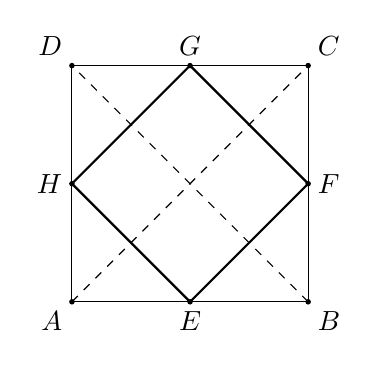
\begin{tikzpicture}[scale=0.5]
  \coordinate (A) at (0,0); \coordinate (B) at (6,0); \coordinate (C) at (6,6); \coordinate (D) at (0,6);
  \coordinate (E) at (3,0); \coordinate (F) at (6,3); \coordinate (G) at (3,6); \coordinate (H) at (0,3);
  \draw (A)--(B)--(C)--(D)--cycle;
  \draw[dashed] (A)--(C) (B)--(D);
  \draw[thick] (E)--(F)--(G)--(H)--cycle;
  \foreach \p/\pos in {A/below left,B/below right,C/above right,D/above left,E/below,F/right,G/above,H/left}\fill(\p)circle(2pt)node[\pos]{$\p$};
\end{tikzpicture}
\end{center}

  \answerarea[46mm]
\end{problem}



\end{document}
